\newcommand{\pdftitel}{Cimarron Herget 2017}
\newcommand{\autor}{Marius Herget}
\newcommand{\version}{draft} % change to "final" to disable comments | "draft" shows notes/tbds/etc
\newcommand{\isPrintVersion}{true}

\documentclass[%
	pdftex,
	oneside,        % Einseitiger Druck.
	12pt,           % Schriftgroesse
	parskip=half,   % Halbe Zeile Abstand zwischen Absätzen.
	headsepline,    % Linie nach Kopfzeile.
	footsepline,    % Linie vor Fusszeile.
	english,        % Translator
]{article}


\usepackage[utf8]{inputenc}
\usepackage[english]{babel}
\usepackage[english]{isodate}
\usepackage[parfill]{parskip}

\usepackage[inline]{enumitem}


\usepackage{ltablex} % mix out of tabularx and longtable
\usepackage{multirow}

\usepackage{graphicx}
\usepackage{wrapfig}
\usepackage{subcaption} %To create subfigures
% \usepackage{subfig} %To create subfigures
\usepackage{placeins} % FloatBarrier
\usepackage{floatrow}
\graphicspath{ {./images/} }

\usepackage[]{geometry}
\usepackage{pdflscape}
\usepackage{booktabs}

\usepackage[most]{tcolorbox}
\usepackage{cleveref}
\usepackage{tikz}
\usetikzlibrary{decorations.pathreplacing,shapes,arrows,positioning}
\usetikzlibrary{positioning}
\usetikzlibrary{backgrounds}
\usetikzlibrary{patterns}

\tikzstyle{input} = [coordinate]
\tikzstyle{output} = [coordinate]
\tikzstyle{block} = [rectangle, draw, text width=5em, text centered,  minimum height=4em]
\tikzstyle{storage} = [cylinder, shape border rotate=90, aspect=0.25, draw]
\tikzstyle{label} = [text width=2.4cm, text centered]
\tikzstyle{wideblock} = [rectangle, draw, text width=7em, text centered,  minimum height=4em]

\usepackage[absolute]{textpos}
\setlength{\TPVertModule}{1mm}
\setlength{\TPHorizModule}{1mm}
\usepackage[\version, layout={inline,index}, singleuser]{fixme}
% Side characters
\newcommand{\impmark}{\strut\vadjust{\domark}}
\newcommand{\domark}{%
	\vbox to 0pt{
		\kern-\dp\strutbox
		\smash{\llap{*\kern1em}}
		\vss
	}%
}
\newcommand{\impquest}{\strut\vadjust{\doquest}}
\newcommand{\doquest}{%
	\vbox to 0pt{
		\kern-\dp\strutbox
		\smash{\llap{?\kern2em}}
		\vss
	}%
}
% Fixme
\fxsetup{envlayout=plain}

\usepackage[backend=bibtex,style=numeric]{biblatex}
\addbibresource{lib/research.bib}


\begin{document}
% TBD
\newcommand{\tbd}[1][null]{
    \ifthenelse{\equal{#1}{null}}
    {\ignorespaces\textit{\impmark\color{orange}\textbf{TBD}}}
    {\ignorespaces\textit{\impmark\color{orange}[TBD: #1]}}
}
\newcommand{\todo}[1][null]{
    \ifthenelse{\equal{#1}{null}}
    {\ignorespaces\textit{\impmark\color{orange}\textbf{TBD}}}
    {\ignorespaces\textit{\impmark\color{orange}[TBD: #1]}}
}



% \maketitle\tableofcontents\newpage
\pagenumbering{Roman}
\title{\textbf{Cimarron}\\Stabilisation of videos in modern \texttt{C++}}
\date{\today}
\author{    Marius Herget\\[2em]
            % {\small Practical Course}\\
            % \textbf{Advanced Software Development with Modern \texttt{C++}}\\
            \textit{in partnership with}\\[2em]
            \textit{Institute for Computer Science}\\
            \textit{Ludwig-Maximilians-Universit\"at M\"unchen}\\[3em]
            
\includegraphics[scale=0.5]{lmu-siegel}}
% (feature abused for this document to repeat the title also on left hand pages)
\maketitle
\newpage
% \tableofcontents
% \newpage
% \listoffigures
% \newpage
% \listoftables
\pagenumbering{arabic}

\section{Idea}
Video stabilization is used ever since cameras evolved. In the early days physicial stabilization techniques as tripods were used. In the following centuries cameras enhanced step by step. New solid and dynamic methods were invented like steady cams, dollys, shoulder rigs and many more. With the invention of digital photography and videos another possible solutionwas found: digital image stabilization. Different techniques like optical flow analysis or warp stabilization were developed. \texttt{Cimarron} implements such a feature tracking method for motion compensation.

\section{Theoratical introduction}
New technologies emerge each year. In the last years espacially phones and small cameras were published. Under ideal condition recent smartphone's cameras pictures cannot be distinguished from professional cameras anymore. Nevertheless, a smartphone video is often detectable by its \textit{handheld}, shaky look. As already mentioned within the short introduction different methods can be used to compensate this motion.

The general idea of video stabilization is to counter, smoothen or to minimize unwanted shakes. In general video motion stabilization can be classified in three categories: mechanical based, optical based and electronical based. Instead of using specific hardware like the first two methods, the electronical approach uses computing power to implement image processing techniques in the  postproduction step. \cite{blockTang}

In order to compensate the unwanted movement of the camera motion can be described in various forms. \textit{Translation} is the simplest form of expression. In this concept direct, linear movement of a single point is described as the distance it covered within a certain time. This can enhanced with the combination of \textit{rotational motion}.  In comparision to translational movement it specifies the angle a point / body covers in a given timeframe. Examples can be seen in \cref{fig:motionmodels}.
\begin{figure}\centering
    \begin{minipage}{.45\textwidth}\centering
        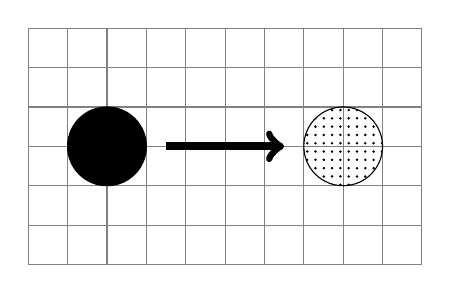
\begin{tikzpicture}[scale=1]
        \draw[step=0.5cm,gray,thin] (-3,-2) grid (2,1);
        \draw[black, fill = black] (-2,-0.5) circle [radius=.5];
        \draw[black, pattern=dots] (1,-0.5) circle [radius=.5];
        \draw[thick, black, ->, line width=1mm] (-1.25,-0.5) -- (0.25,-0.5);
        \end{tikzpicture}
        \subcaption{Translational motion}
    \end{minipage}
    \begin{minipage}{.45\textwidth}\centering
        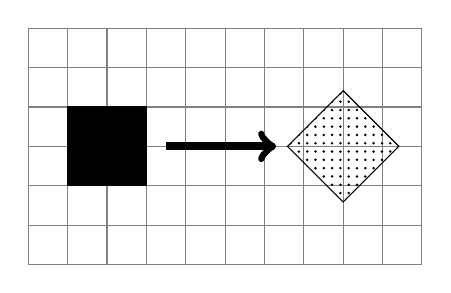
\begin{tikzpicture}[scale=1]
        \draw[step=0.5cm,gray,thin] (-3,-2) grid (2,1);
        \draw[black, fill = black] (-2.5,0) rectangle (-1.5,-1);
        \draw[black, pattern=dots,rotate around={45:(1,-0.5)}] (0.5,0) rectangle (1.5,-1);
        \draw[thick, black, ->, line width=1mm] (-1.25,-0.5) -- (0.15,-0.5);
        \end{tikzpicture}
        \subcaption{Rotational motion}
    \end{minipage}
    \caption{Differnt motion models}
    \label{fig:motionmodels}
\end{figure}


\begin{landscape}
    % \section{System diagram}
    \begin{figure}[h!]
% \centered
\small
\begin{tikzpicture}[node distance=1cm and 2cm,auto]
    \node [input, name=input] {};
    \node [block, right= of input] (pre1) {\textbf{Decoding} Extracting frames};
    \node [block, right= of pre] (analysis1) {\textit{\tiny Local Motion Estimation:} CAMShift Tracking};
    \node [block, right= of analysis1] (analysis2) {\textit{\tiny Motion Aggregation:} CompareTrackingVectors};
    \node [block, right= of analysis2] (analysis3) {\textit{\tiny Motion Analysis:} Filter Tracking Errors};
    \node [block, below= of analysis3] (analysis3) {\textit{\tiny Global Motion Analysis:} Aggregation to global motion data};
    \node [block, left= of analysis3] (stabi) {\textit{\tiny Stabilization:} Transform frames};
    \node [block, left= of stabi] (post1) {\textit{\tiny Post-processing:} Reframe image};
    \node [block, left= of post1] (post2) {Encoding};
    \node [input, left=of post2] (output) {t};

    \node [storage, below right=0.5cm and 0.7cm of analysis] (analysisstorage) {DB};

     \draw[->](input) -- node {Video}(pre);
     \draw[->](analysis1) -- node {Motion Tracking Data}(analysis2);
     \draw[->](analysis1) -- node {\tiny Correctiondata} node[below]{m(n) = TV(n)}(analysis2);

     \draw[->](post) -- node {Video}(output);
\end{tikzpicture}
\caption{High-level system diagram}
\end{figure}

    % \begin{figure}[h!]
% \centered
\small
\begin{tikzpicture}[node distance=1cm and 2cm,auto]
    \node [input, name=input] {};
    \node [block, right= of input] (pre1) {\textbf{Decoding} Extracting frames};
    \node [block, right= of pre] (analysis1) {\textit{\tiny Local Motion Estimation:} CAMShift Tracking};
    \node [block, right= of analysis1] (analysis2) {\textit{\tiny Motion Aggregation:} CompareTrackingVectors};
    \node [block, right= of analysis2] (analysis3) {\textit{\tiny Motion Analysis:} Filter Tracking Errors};
    \node [block, below= of analysis3] (analysis3) {\textit{\tiny Global Motion Analysis:} Aggregation to global motion data};
    \node [block, left= of analysis3] (stabi) {\textit{\tiny Stabilization:} Transform frames};
    \node [block, left= of stabi] (post1) {\textit{\tiny Post-processing:} Reframe image};
    \node [block, left= of post1] (post2) {Encoding};
    \node [input, left=of post2] (output) {t};

    \node [storage, below right=0.5cm and 0.7cm of analysis] (analysisstorage) {DB};

     \draw[->](input) -- node {Video}(pre);
     \draw[->](analysis1) -- node {Motion Tracking Data}(analysis2);
     \draw[->](analysis1) -- node {\tiny Correctiondata} node[below]{m(n) = TV(n)}(analysis2);

     \draw[->](post) -- node {Video}(output);
\end{tikzpicture}
\caption{High-level system diagram}
\end{figure}

\end{landscape}
\section{Coding Concepts}
\begin{description}
    \item[preprocessing]
    \begin{table}[ht]
    \begin{tabular}{@{}llll@{}}
    \toprule
    \textbf{Expression} & \textbf{Return} & \textbf{Equivalent expression} & \textbf{Notes} \\ \midrule
       &                 &                                &                \\
                    &                 &                                &                \\ \bottomrule
    \end{tabular}
    \end{table}
\end{description}



\printbibliography\cleardoublepage

\end{document}
